% TeX encoding = utf8
% TeX spellcheck = pl_PL 
\documentclass[a4paper, 11pt]{article}
\usepackage[utf8]{inputenc}
\usepackage[polish]{babel}
\usepackage{polski}
\usepackage{float}
\usepackage{graphicx}
\usepackage{listings}
\usepackage{amsfonts}
\usepackage{geometry}
\usepackage{multicol}
\usepackage{latexsym}
\usepackage{enumerate}
\usepackage{hyperref}
\usepackage{wrapfig}
\usepackage{color} %red, green, blue, yellow, cyan, magenta, black, white
\definecolor{mygreen}{RGB}{28,172,0} % color values Red, Green, Blue
\definecolor{mylilas}{RGB}{170,55,241}

\author{Kamil Foryszewski}
\title{Sterowanie Procesami - projekt I, zadanie 1.33}
\frenchspacing

\newgeometry{tmargin=2cm, bmargin=2cm, lmargin=2cm, rmargin=2cm}
\pagestyle{empty}


\begin{document}

\lstset{language=Matlab,%
    basicstyle=\color{red},
    breaklines=true,%
    morekeywords={matlab2tikz},
    keywordstyle=\color{blue},%
    morekeywords=[2]{1}, keywordstyle=[2]{\color{black}},
    identifierstyle=\color{black},%
    stringstyle=\color{mylilas},%
    commentstyle=\color{mygreen},%
    showstringspaces=false,
    numbers=right,%
    numberstyle={ \color{black}},% size of the numbers
    numbersep=5pt, % this defines how far the numbers are from the text
    emph=[1]{for,endfor,endwhile,endfunction,endif,break},emphstyle=[1]\color{blue}, %some words to emphasise
    emph=[2]{,.}, emphstyle=[2]\color{yellow},%
}

\maketitle
\tableofcontents

\section{Polecenie 1}

\subsection{Ciągły obiekt dynamiczny}
Dany jest ciągły obiekt dynamiczny o transmitancji: 
$$G(s) = \frac{2s^2+22s+48}{s^3+8s^2-65s-504} = \frac{2(s+8)(s+3)}{(s+7)(s-8)(s+9)}$$

\subsection{Transmitancja dyskretna}
Wyznaczona transmitancja dyskretna ma następującą postać: 
$$G(z) = \frac{0.2539z^2-0.3048s+0.0858}{z^3-3.1287z^2-2.2119z-0.4493}$$
Została wyznaczona przy pomocy polecenia \emph{c2d} pakietu matlab. 
$$Gs = tf([2\quad 22\quad 48], [1\quad 8\quad -65\quad -504])$$
Na początku został utworzony model transmitancji ciągłej wykorzystany poźniej do wyznaczenia transmitancji dyskretnej. 
$$Gz = c2d(Gs,0.1,\ 'zoh')$$
Gdzie $0.1$ to okres próbkowania, \emph{'zoh'} oznacza ekstrapolator zerowego rzędu. 
\subsection{Zera i bieguny transmitancji}
Dla transmitancji ciągłej zera i bieguny odczytujemy bezpośrednio ze wzoru:\\
Zera: \\

$s_0^1 = -8$\\

$s_0^2 = 3$\\

\noindent Bieguny: \\

$s_b^1 = -7$\\

$s_b^2 = 8$\\

$s_b^3 = -9$\\
\\
Dla transmitancji dyskretnej zera i bieguny zostały wyznaczone funkcją \emph{roots} pakietu matlab:\\ 
Zera:\\

$z_0^1=0.7502$\\

$z_0^2=0.4502$\\

\noindent Bieguny:\\

$z_b^1 = 2.2255$\\

$z_b^2 =0.4966$\\

$z_b^3 =0.4066$


\subsection{Stabilnosć}
Na podstawie wartości biegunów transmitancj ciągłej, możemy stwierdzić że układ jest niestabilny. Wynika to z dotatniej wartości jednego z biegunów, co nie jest zgodne z warunkiem stabilności asymptotycznej. Podobnie dla transmitancji dyskretnej, odległość od początku układu współrzędnych na płaszczyźnie zespolonej powinna być mniejsza niż 1. Warunku tego nie spełnia jeden z biegunów. 

\section{Reprezentacja modelu dyskretnego w przestrzeni stanów}
\subsection{Wyznaczanie parametrów modelu}
Do określenia modelu w przestrzeni stanu na podstawie transmitancji wykorzystano funkcję \emph{tf2ss}:\\
\\
\indent $A= \left[
        \begin{array}{ccc}
         3.1287	&-2.2119	&0.4493\\
         1	&0	&0\\
		 0 & 1&	0
         \end{array}
      \right]$
$B= \left[
        \begin{array}{c}
         1\\
         0\\
         0
         \end{array}
      \right]$
$C= \left[
        \begin{array}{ccc}
         0.2539&-0.3048	&0.0858\\
         \end{array}
      \right]$
$D=0$\\
\\
\\
Stosując drugą metodę bezpośrednią:\\
\\

$A_1= \left[
        \begin{array}{ccc}
		3.1287	&1	&0\\
		-2.2119	&0	&1\\
		0.4493	&0	&0
         \end{array}
      \right]$
$B_1= \left[
        \begin{array}{c}
		0.2539\\
		-0.3048\\
		0.0858
         \end{array}
      \right]$
$C_1= \left[
        \begin{array}{ccc}
         1&0&0\\
         \end{array}
      \right]$
$D_1=0$\\
\\

\noindent Równania stanu dla metody II mają postać:
\\

$x_1(k+1) = 3.1287x_1(k)+x_2(k)+ 0.2539u(k)$ \\
\indent$x_2(k+1) = -2.2119x_1(k)+x_3(k)-0.3048u(k)$ \\
\indent$x_3(k+1) = 3.1287x_1(k)+ 0.0858u(k)$ \\
\indent$y(k) = x_1(k)$ \\

\subsection{Reprezentacja graficzna modelu}
\begin{figure}[H]
\centering
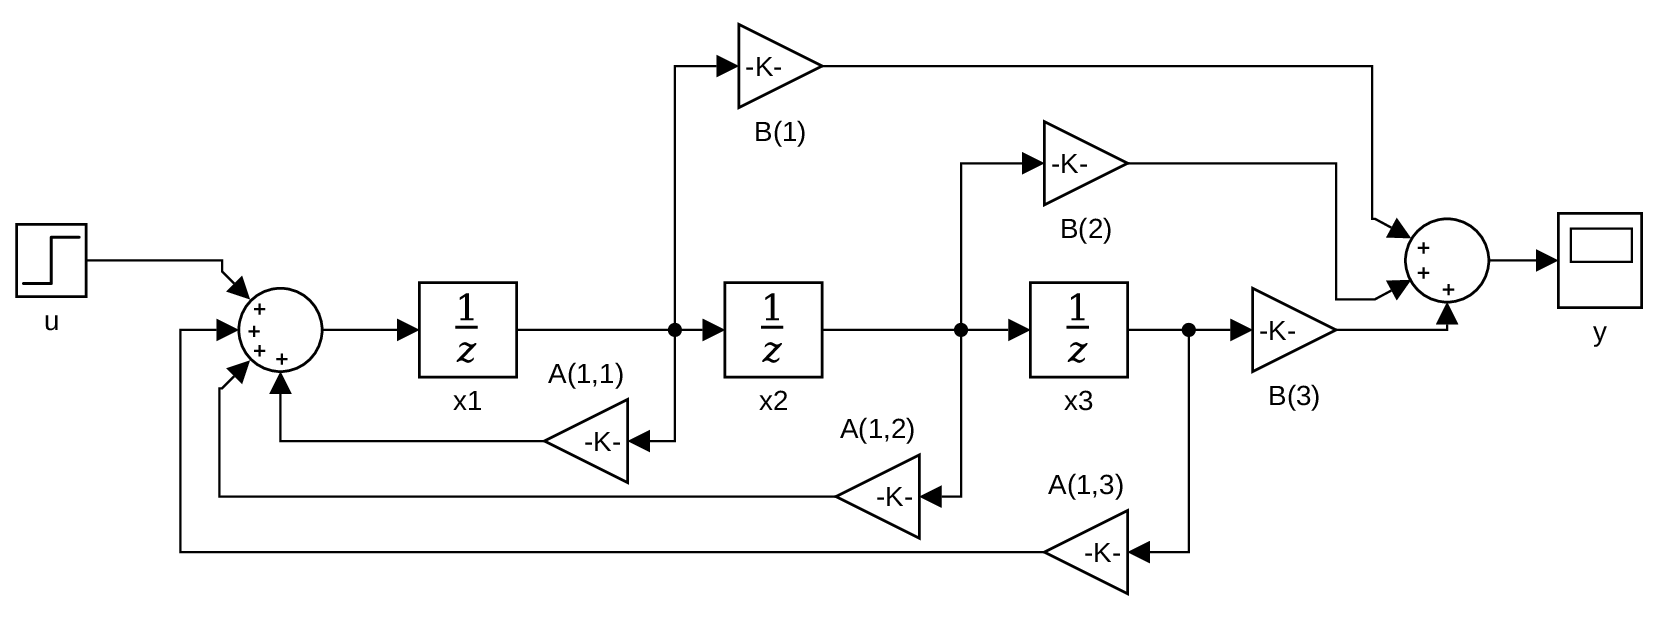
\includegraphics[scale=0.3]{obiekt2.png}
\caption{Reprezentacja graficzna modelu wariant I metody bezpośredniej}
\end{figure}
\begin{figure}[H]
\centering
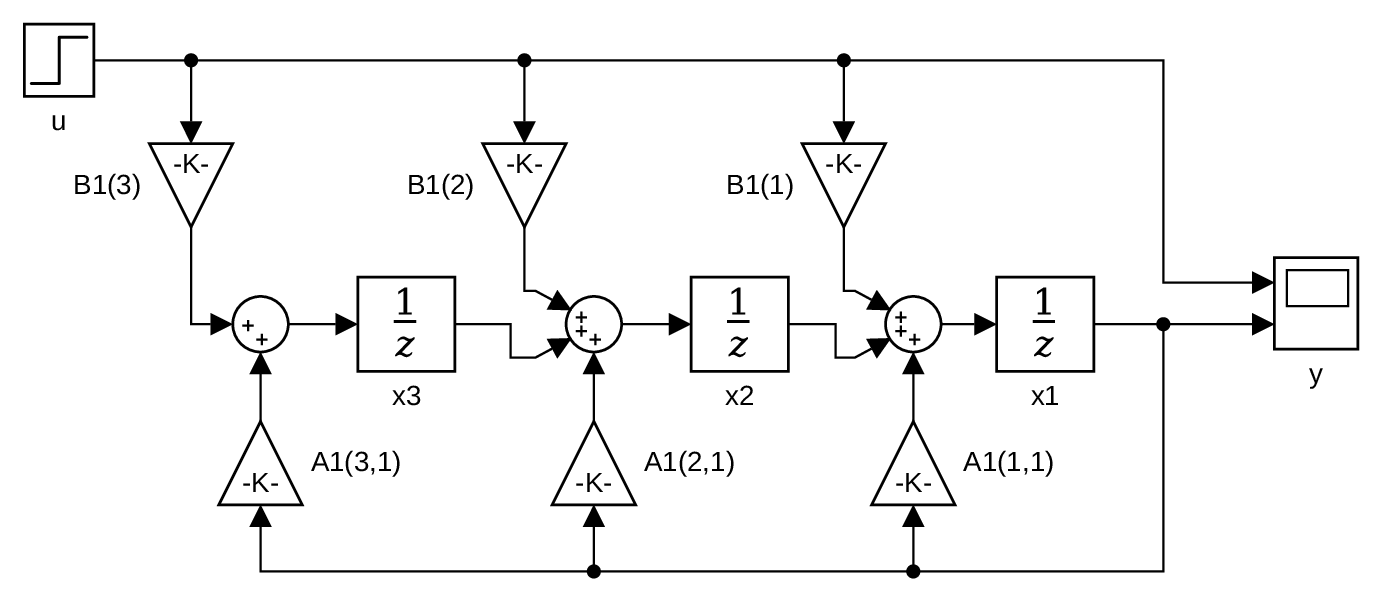
\includegraphics[scale=0.35]{obiekt1.png}
\caption{Reprezentacja graficzna modelu wariant II metody bezpośredniej}
\end{figure}

\section{Regulator ze zprzężanem od stanu}
Zadaniem regulatora ze sprzężenieim od stanu jest sprowadzenie procesu od stanu początkowego do stanu zerowego. Należy więc wyznaczyć wektor $K$ który zgodnie z prawem regulacji: $u(k) = -Kx(k)$ zapewnidobrą jakość regulacji. 
\subsection{Trzy takie same bieguny rzeczywiste}
W celu ustalenia najlepszego punktu ulokowania wykonam symulacje w zakresie od 0.05 do 0.8 co 0.05. \\

\noindent Wektor K wyznaczymy za pomocą polecenia acker pakietu matlab\\

$K = acker(A_1,B_1,p)$\\

\subsection{Maksymalny przyrost sterowania w zależności od biegunów} 
\begin{figure}[ht]
\centering
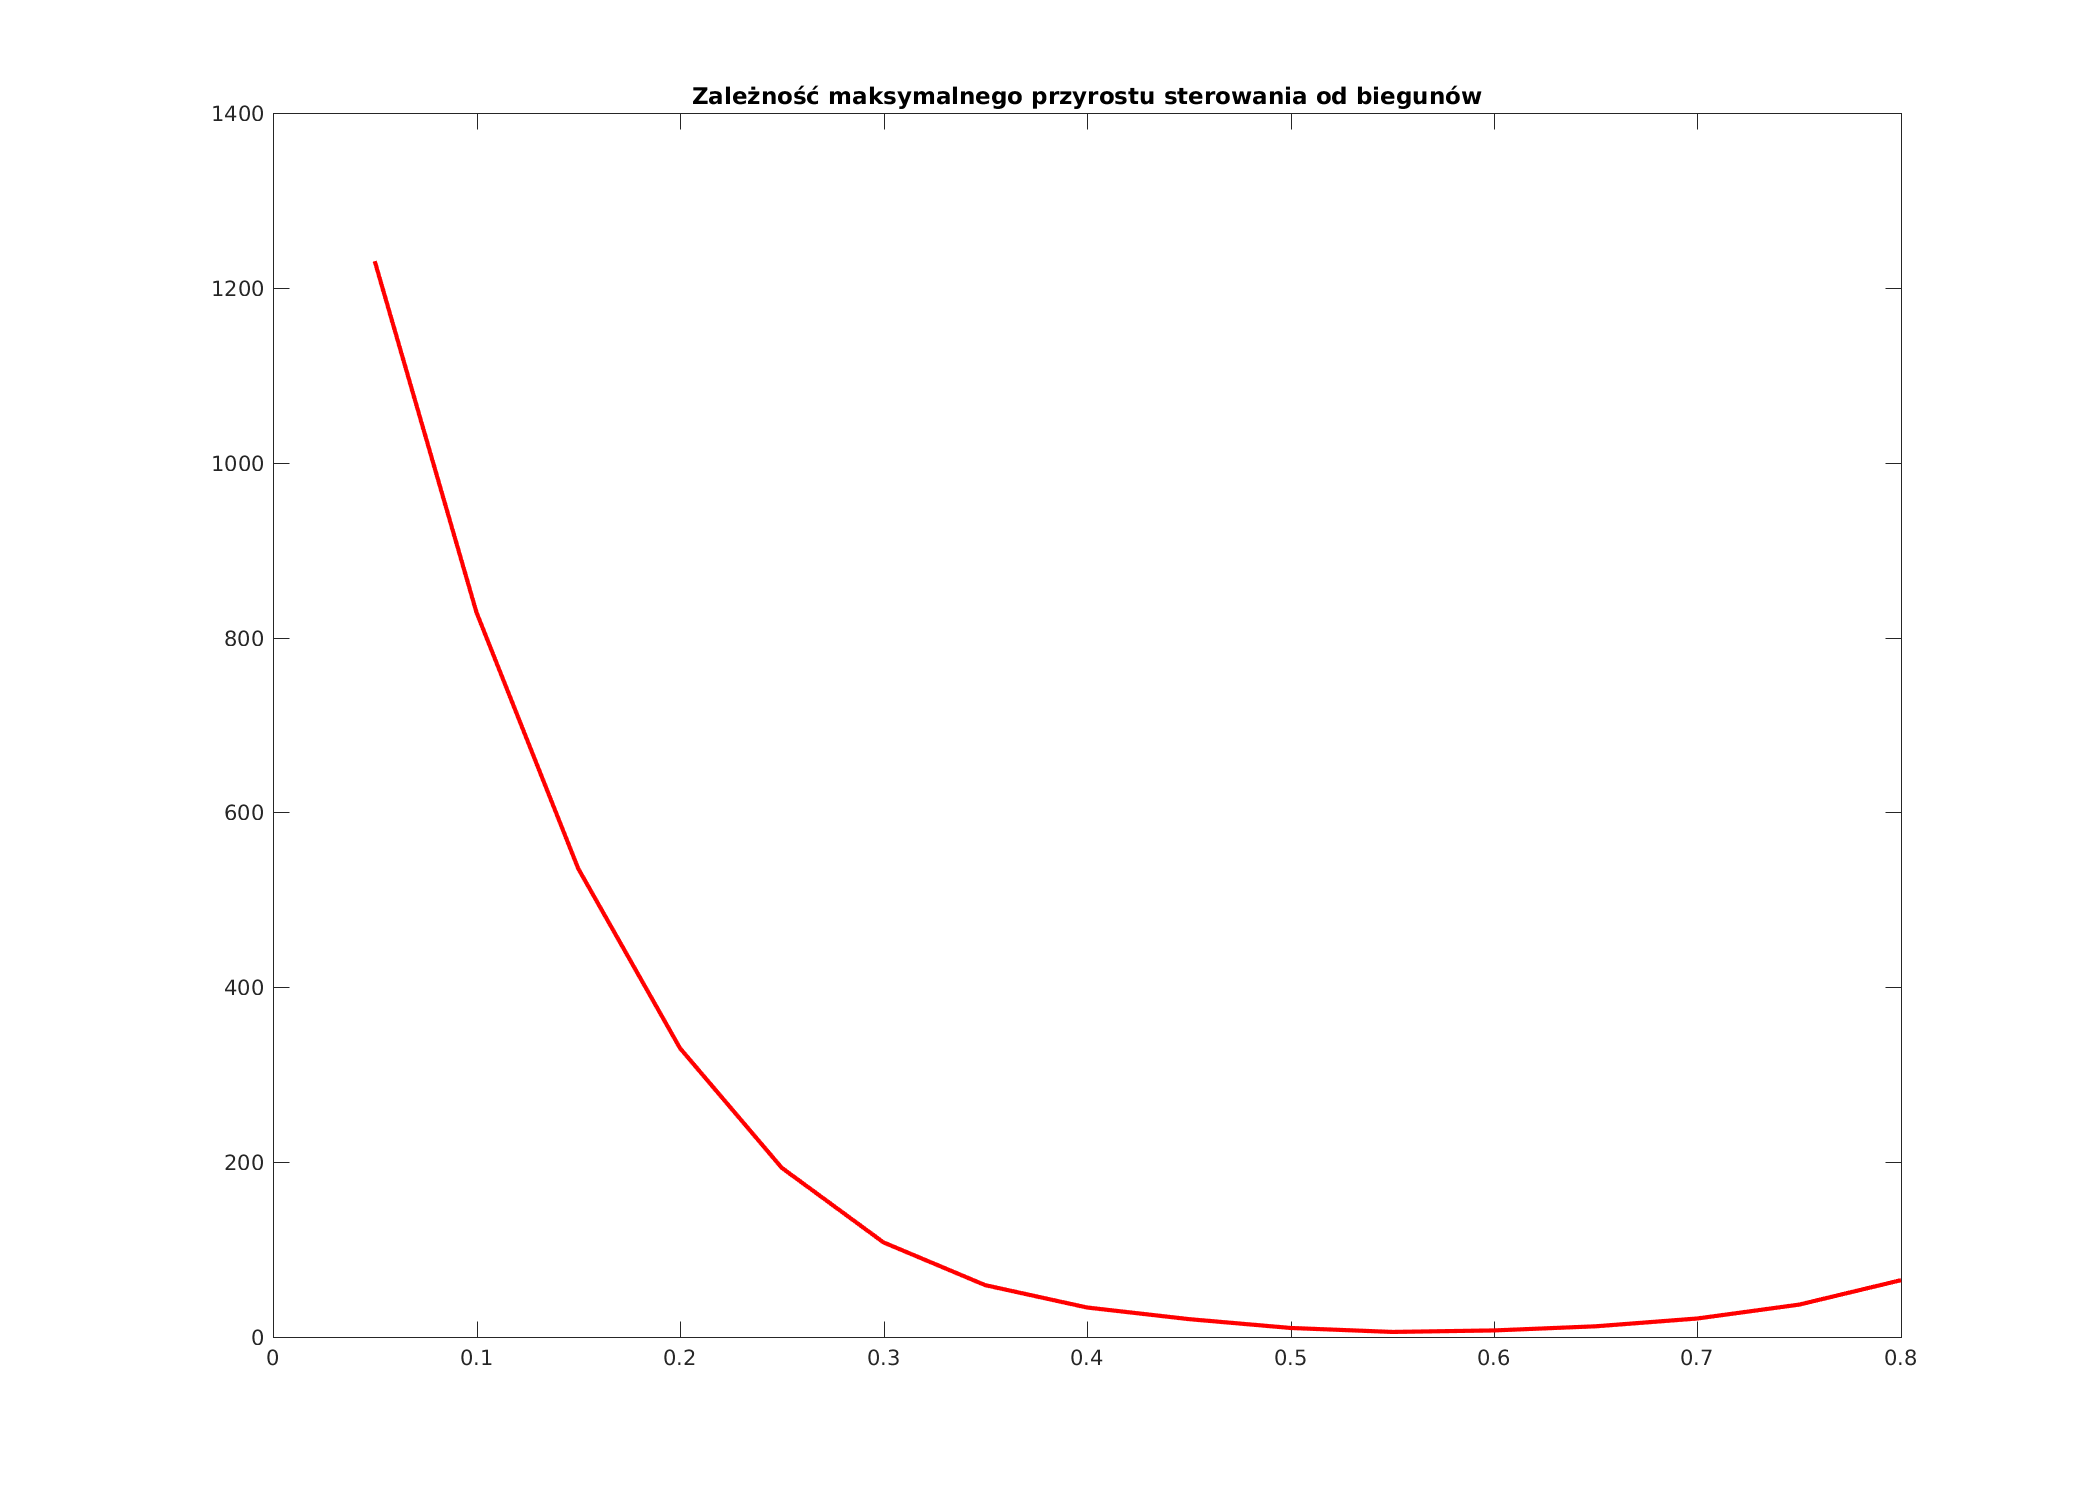
\includegraphics[scale=0.5]{3_1.png}
\caption{Wykrez sależności maksymalnego przyrostu sterowania od wartoości biegunów}
\end{figure}


\noindent Stosując jako wskaźnij jakości minimalny przyrost sterowania możemy odczytać z wykresu lokalizację biegunów, wtedy :\\
\\

$p = [0.55\quad0.55\quad 0.55]$\\

\noindent Co Potwierdza poniższy wykres symulacji. Regulator w którkim czasie i bez sokoków sterowania sprowadza układ do stanu końcowego. 

\begin{figure}[H]
\centering
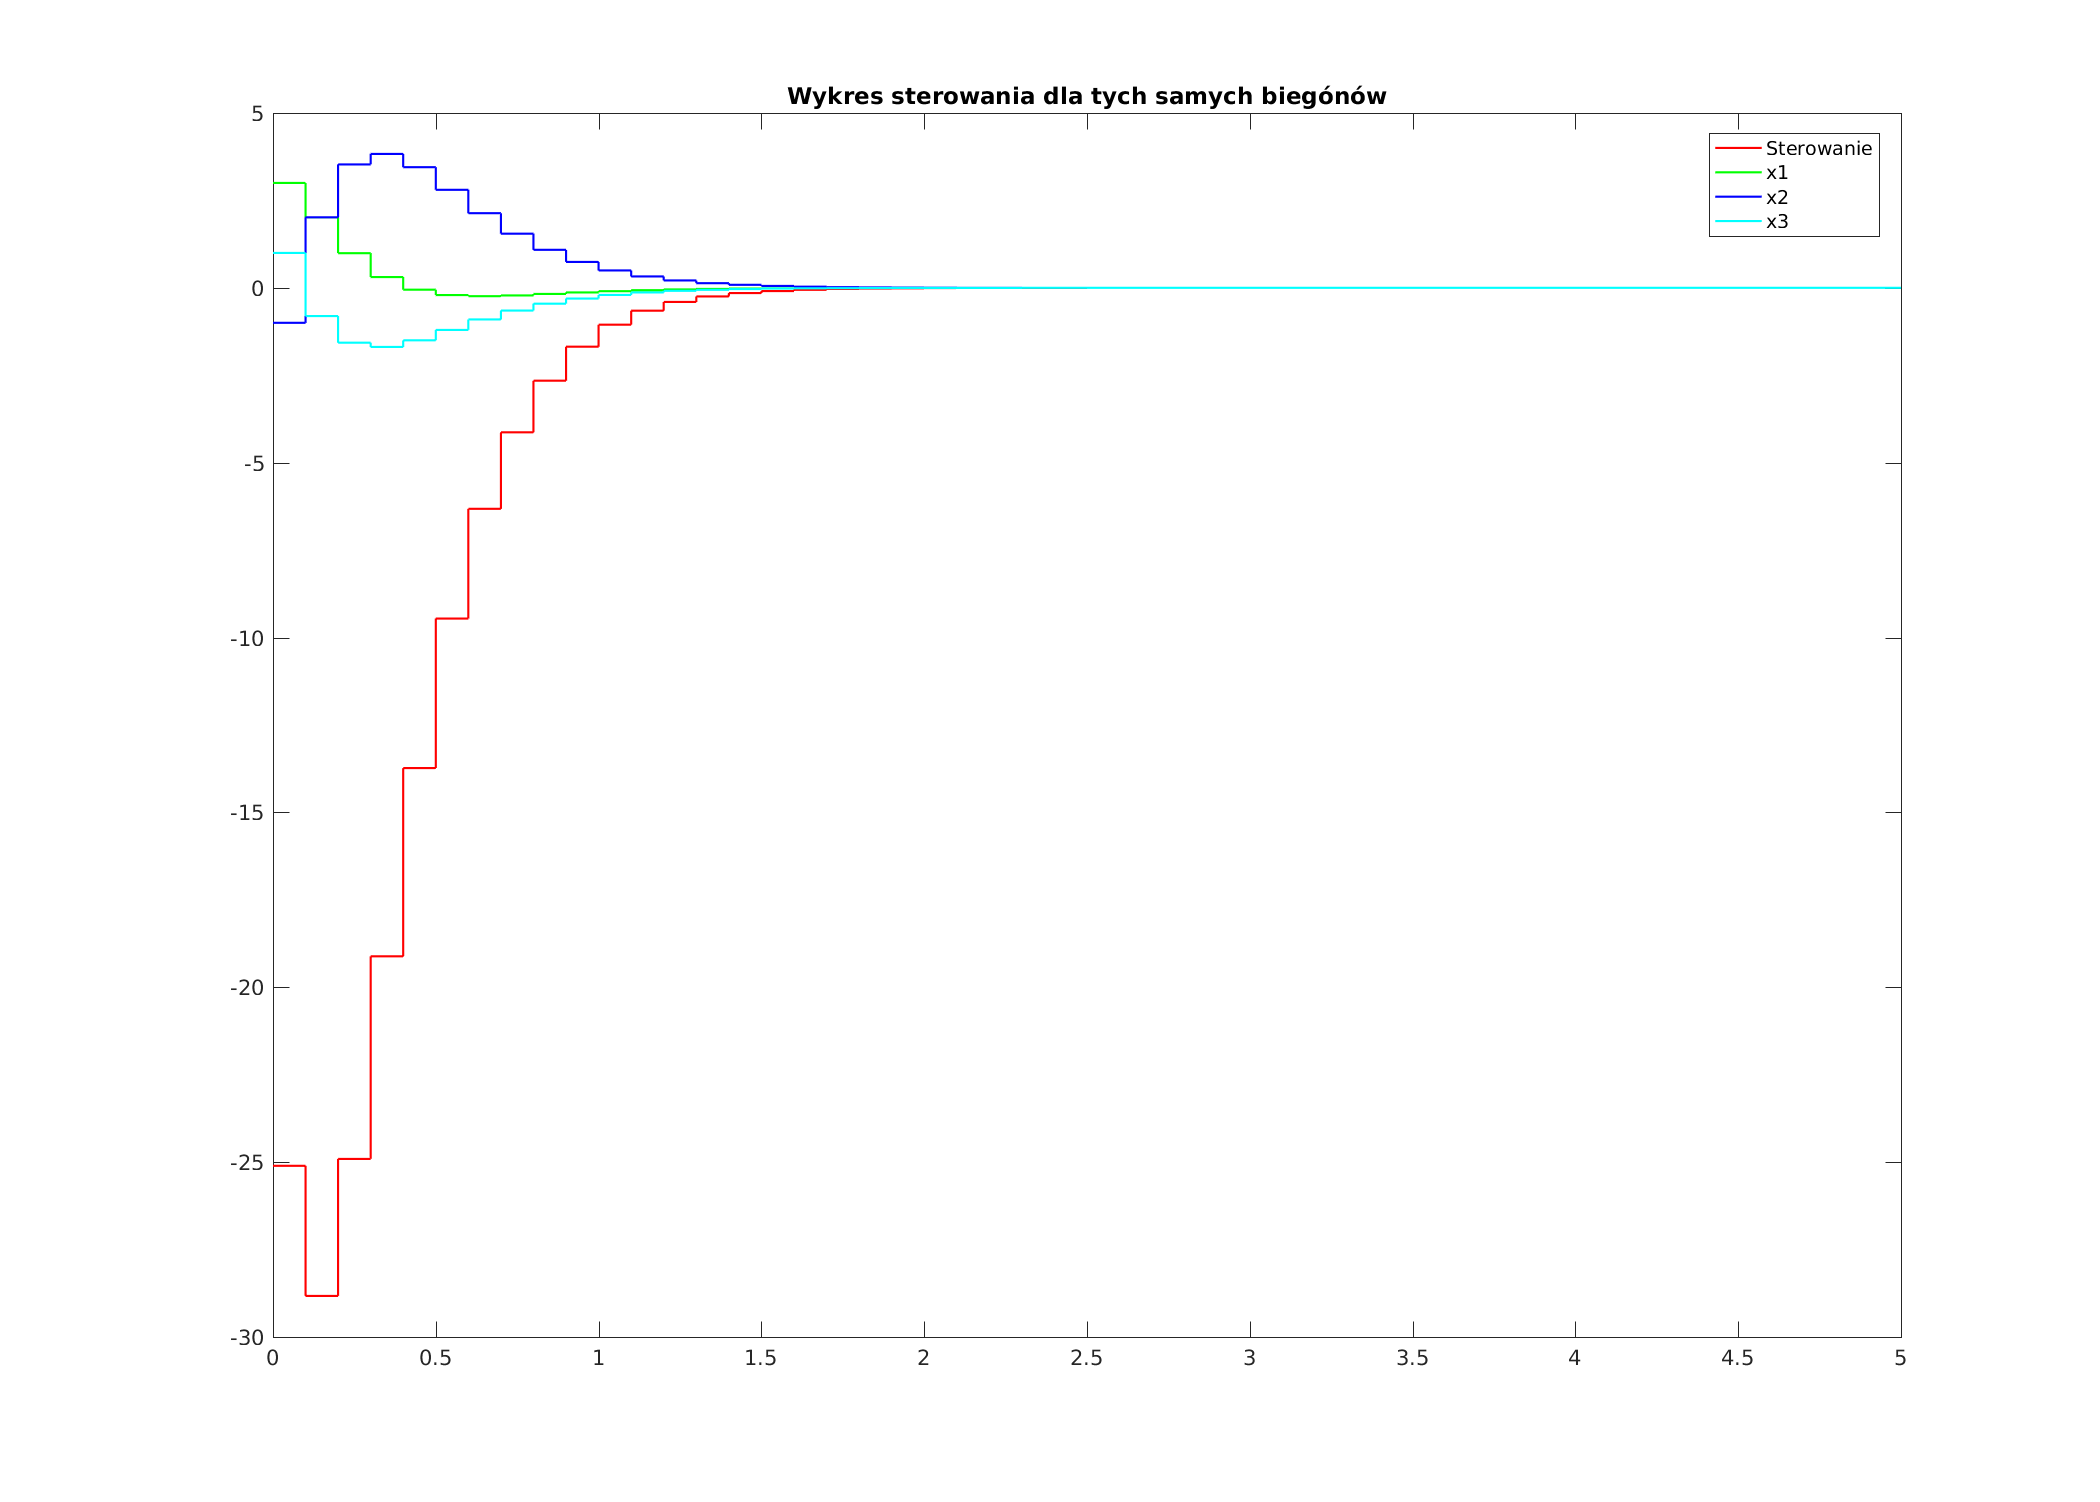
\includegraphics[scale=0.5]{3_t.png}
\caption{Wykres symulacji obiektu dla najlepszego wyboru takich samych biegunów}
\end{figure}

\noindent Wektor K wynosi dla takigo umiejscowienia:\\

$K= \left[
        \begin{array}{ccc}
         17,344&10,505&10,225\\
         \end{array}
      \right]$


\subsection{Biegun dominiujący}
Koljejnym etapem jest takie dobranie biegunów, aby jeden z nich był dominujący, a pozostałe miały jak najmniejsze znaczenie na układ regulacji. Nadal wybieramy spośród prawej połowy koła jednostkowego. Szybkość regulacji zależy od odległosci od środka układu. W przypadku biegunu dominującego należy ulokować dwa bieguny blisko środka układu oraz jeden dominujący znacznie dalej. Zostało przeprowadzonych kilka symulacji spełniających powyższe założenia. Oto najlepsza z nich:\\
\\

$p = [0.4\quad0.4\quad 0.7]$\\

\begin{figure}[H]
\centering
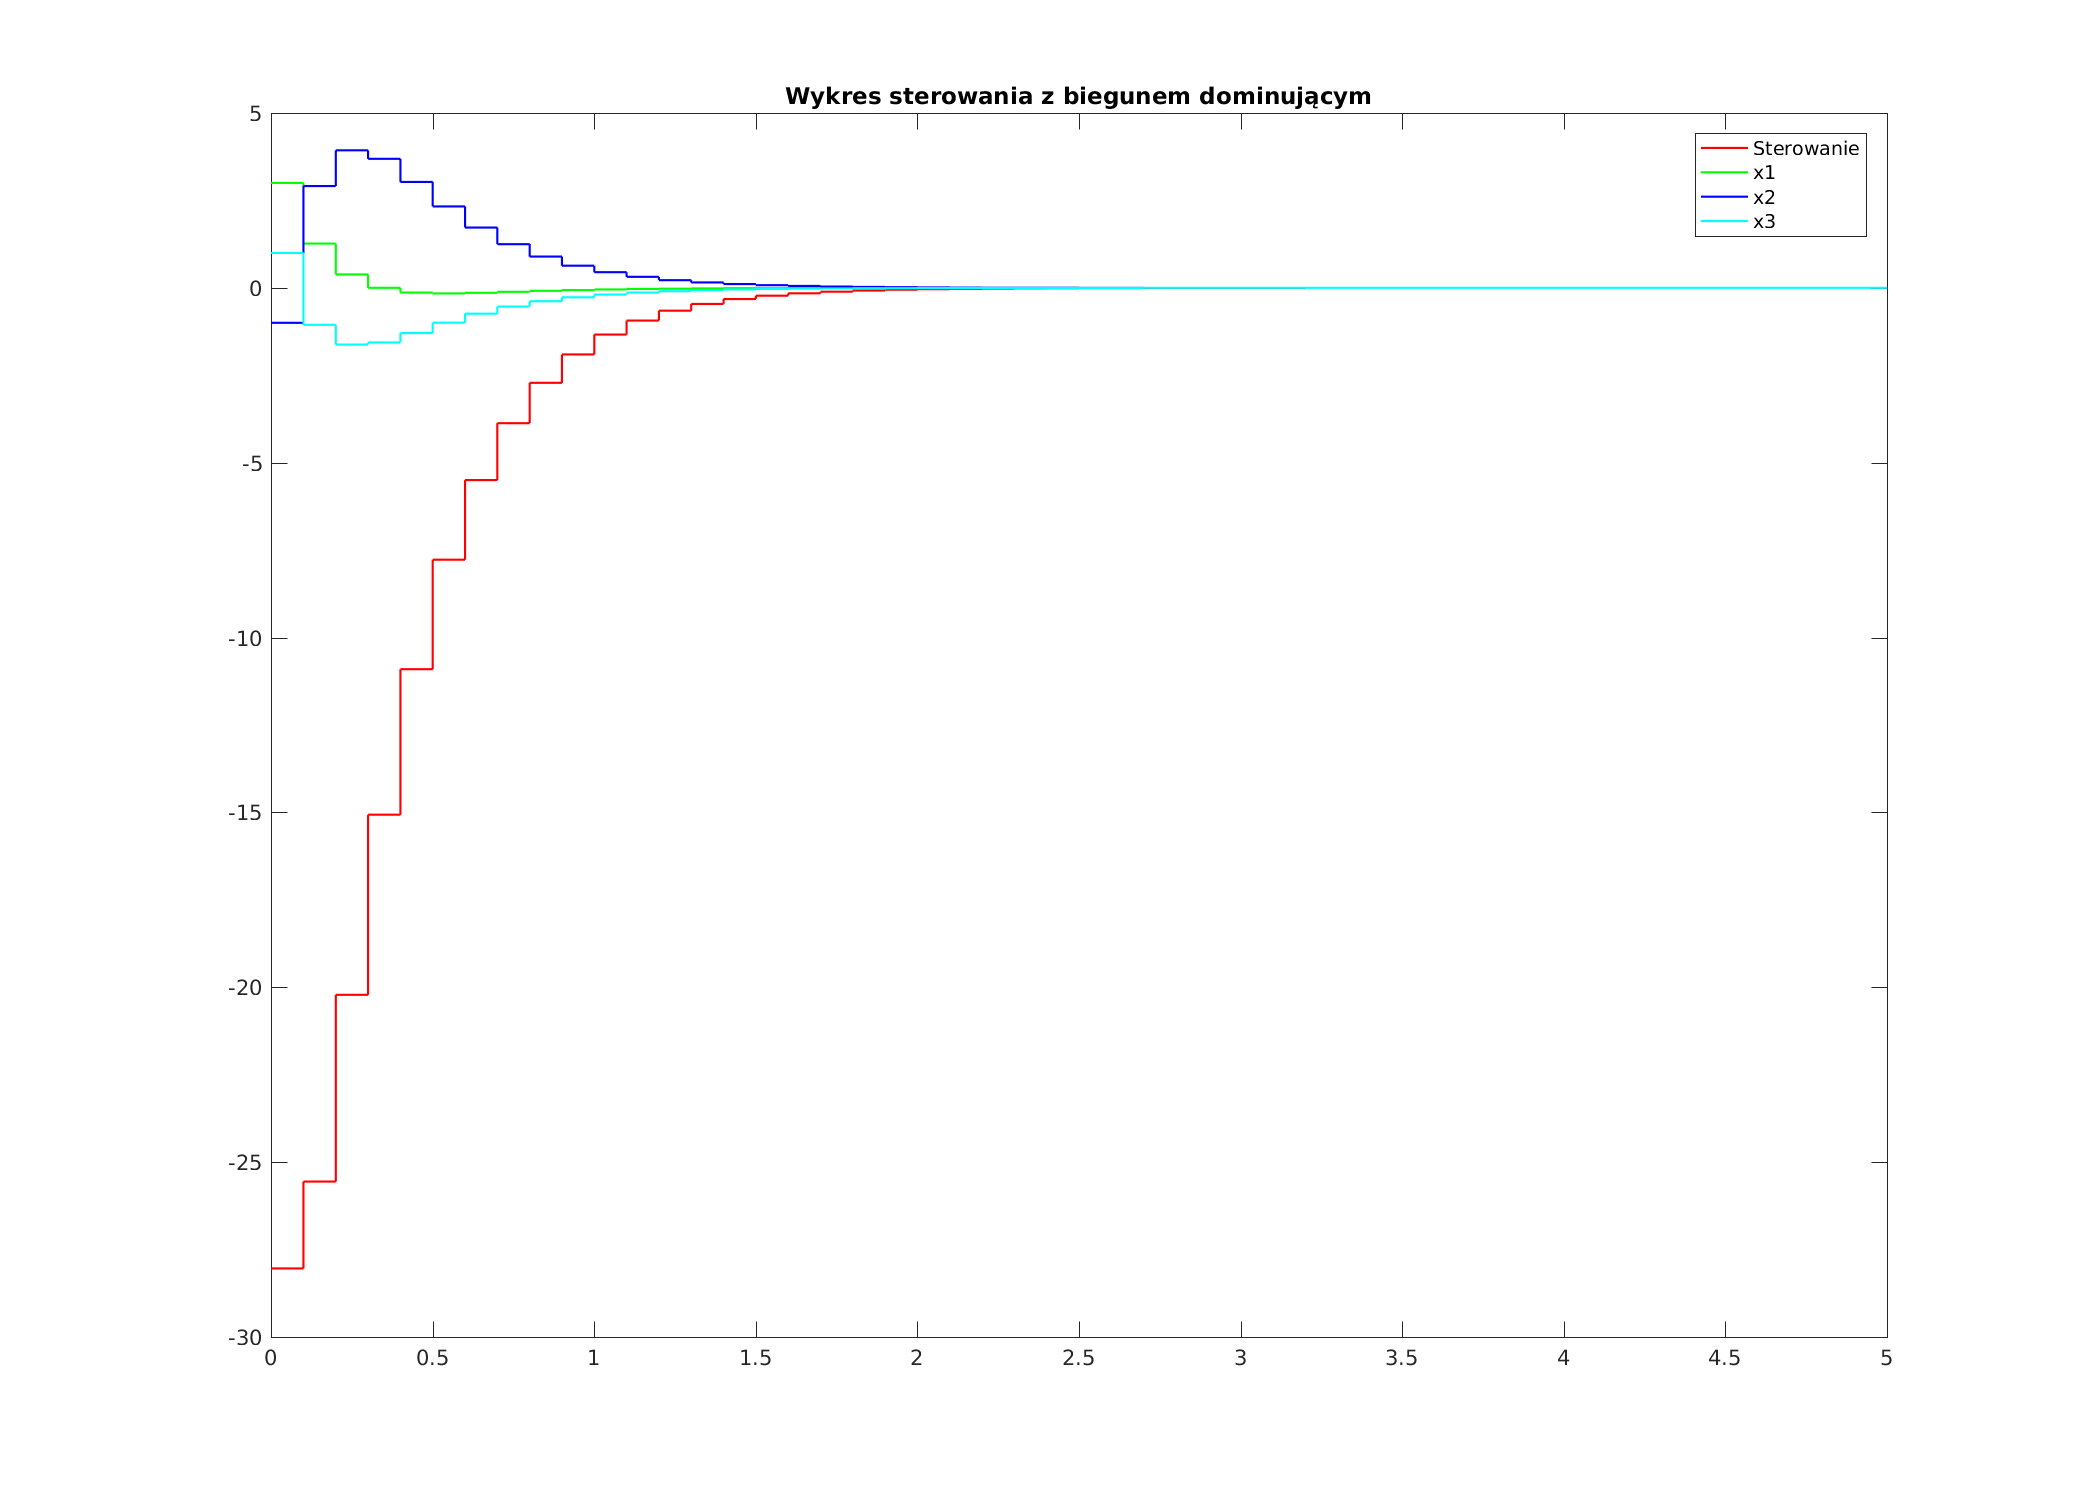
\includegraphics[scale=0.5]{3_d.png}
\caption{Wykres symulacji obiektu dla najlepszego wyboru biegunu dominującego}
\end{figure}


\subsection{Struktura układu regulacji} 
Symulacje zostały przeprowadzone na obiekcie ze sprzężeniem od stanu którego reprezentacja graficzna przedstawiona jest poniżej. 

\begin{figure}[H]
\centering
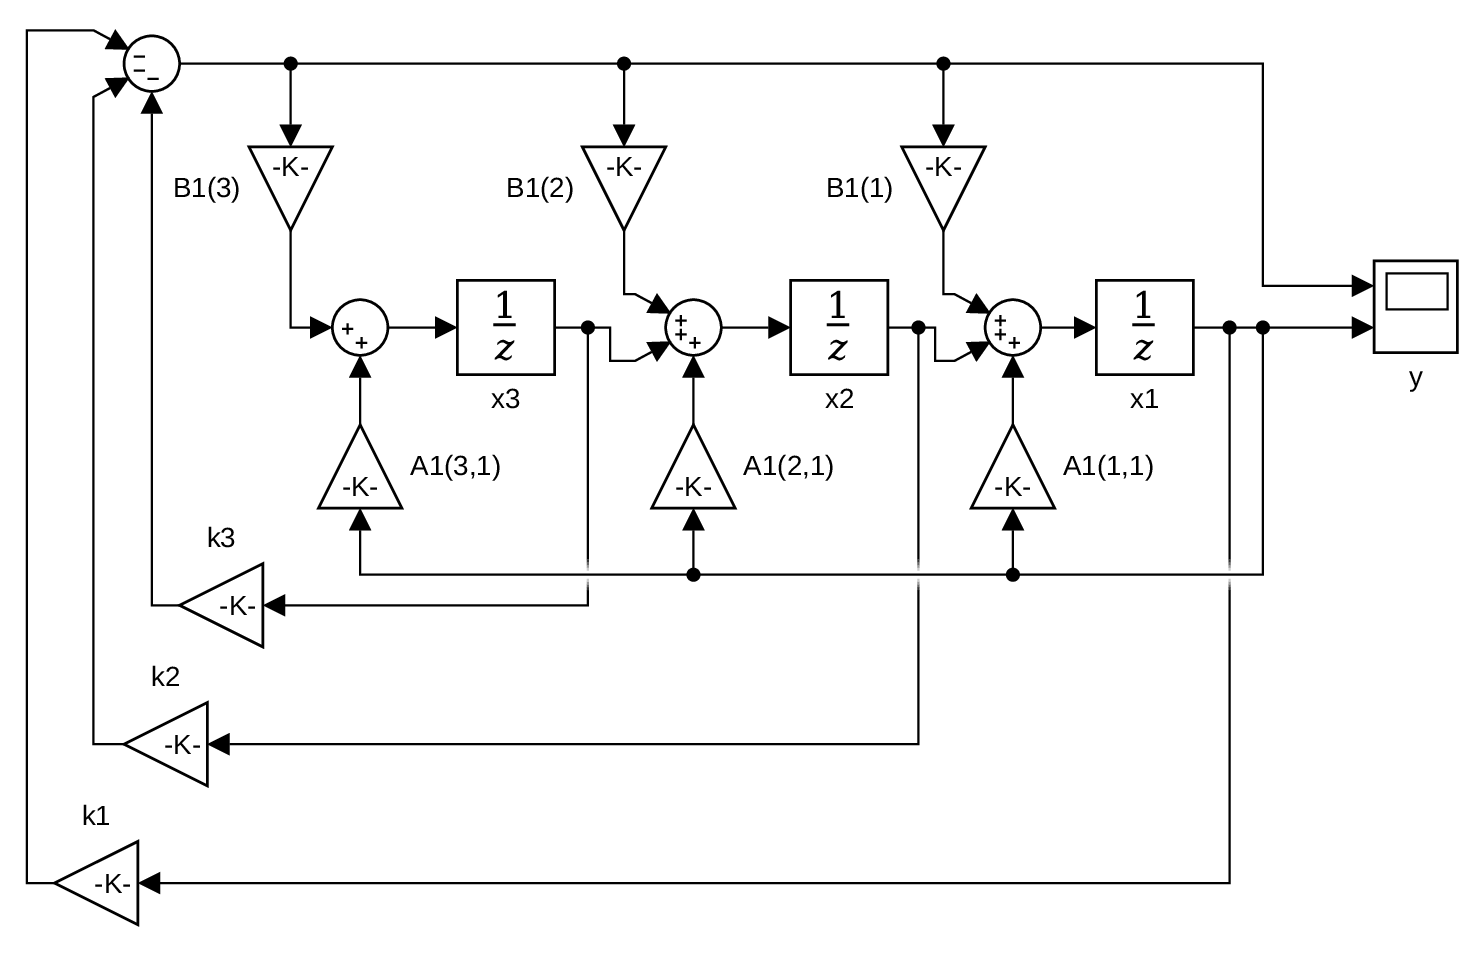
\includegraphics[scale=0.3]{obiekt_regulator.png}
\caption{Struktura obiektu z regulatorem}
\end{figure}

\section{Obserwator zredukowanego rzędu}
\subsection{Ogólna struktura obserwatora zredukowanego rzędu}
\begin{figure}[H]
\centering
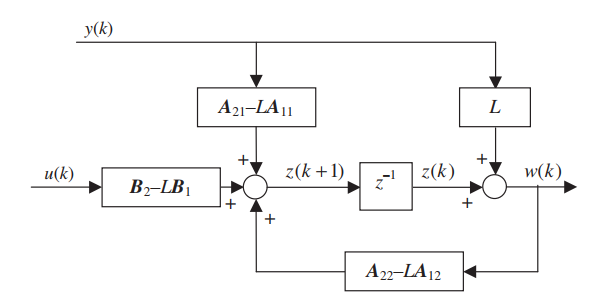
\includegraphics[scale=0.80]{obs.png}
\caption{Ogólna struktura obserwatora zredukowanego rzędu}
\label{}
\end{figure}

\subsection{Wyznaczanie parametrów}
Wektor L oblicza się porównując współczynniki przy odpowiednich potęgach zmiennej $z$
wielomianu charakterystycznego. Wektor L można wyznaczyć korzystając z polecenia pakietu matlab. Szukaną wielkość L znajduje się  następująco:\\

$L=acker(A_{22} ’,A_{12} ’, [z_{o2}\quad z_{o3} ])$\\

\noindent Równanie Obserwatora zredukowanego rzędu ma następującą postać:\\
\\

$z(k=1) = (A_{22}-LA_{12}(z(k)+Ly(k))+(A_{21}-LA_{11})y(k)+(B_2-LB1)u(k)$

\subsection{Reprezentacja graficzna obiektu z obserwatorem}
Na podstawie równania obserwatora został zrealizowany model w Symulinku zawierający obiekt, regulator i obserwator zredukowanego rzędu. Schemat układu znajduje się poniżej: 

\begin{figure}[H]
\centering
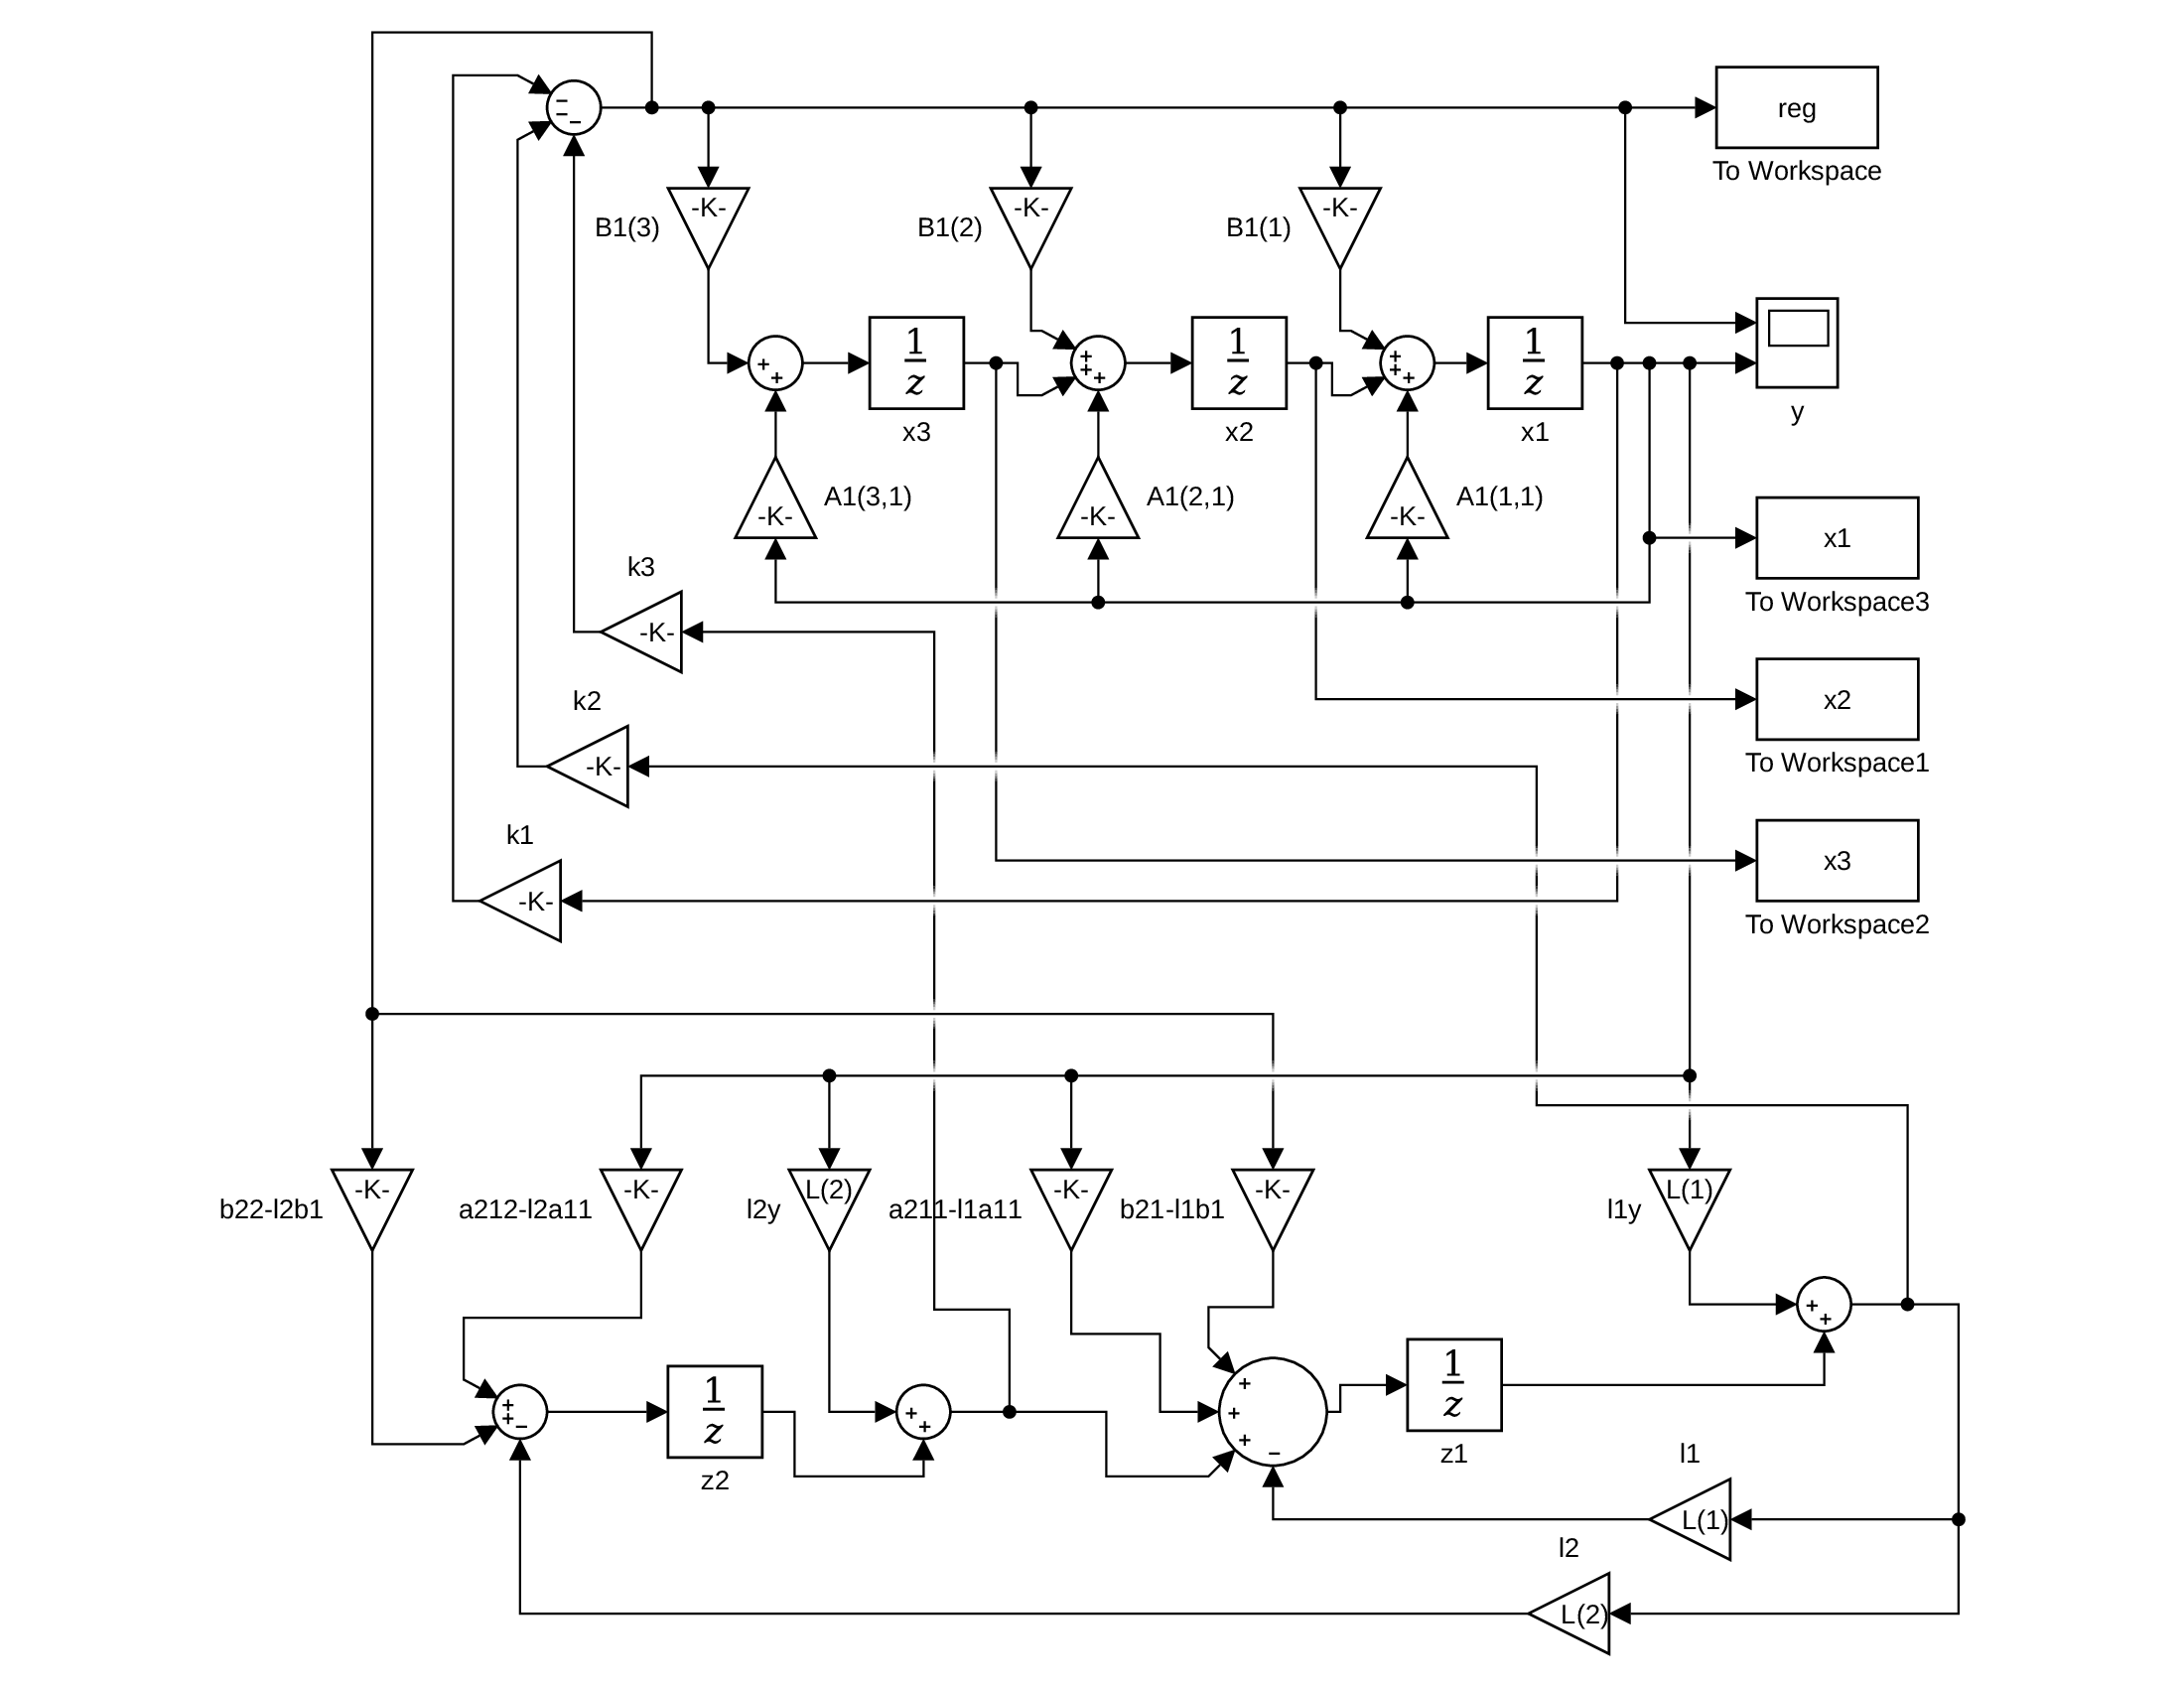
\includegraphics[scale=0.23]{obiekt_obserwator_regulator.png}
\caption{Struktura obiektu z regulatorem i obserwatorem zredukowanego rzędu}
\end{figure}

\subsection{Obserwator wolny}
W pierwszym podpunkcie bieguny obserwatora zostały ulokowane tak, aby regulacja następowała wolno. Najlepszy rezultat z symulowanych wystąpił dla wektora: \\

$p = [0.8\quad0.8]$\\

\begin{figure}[H]
\centering
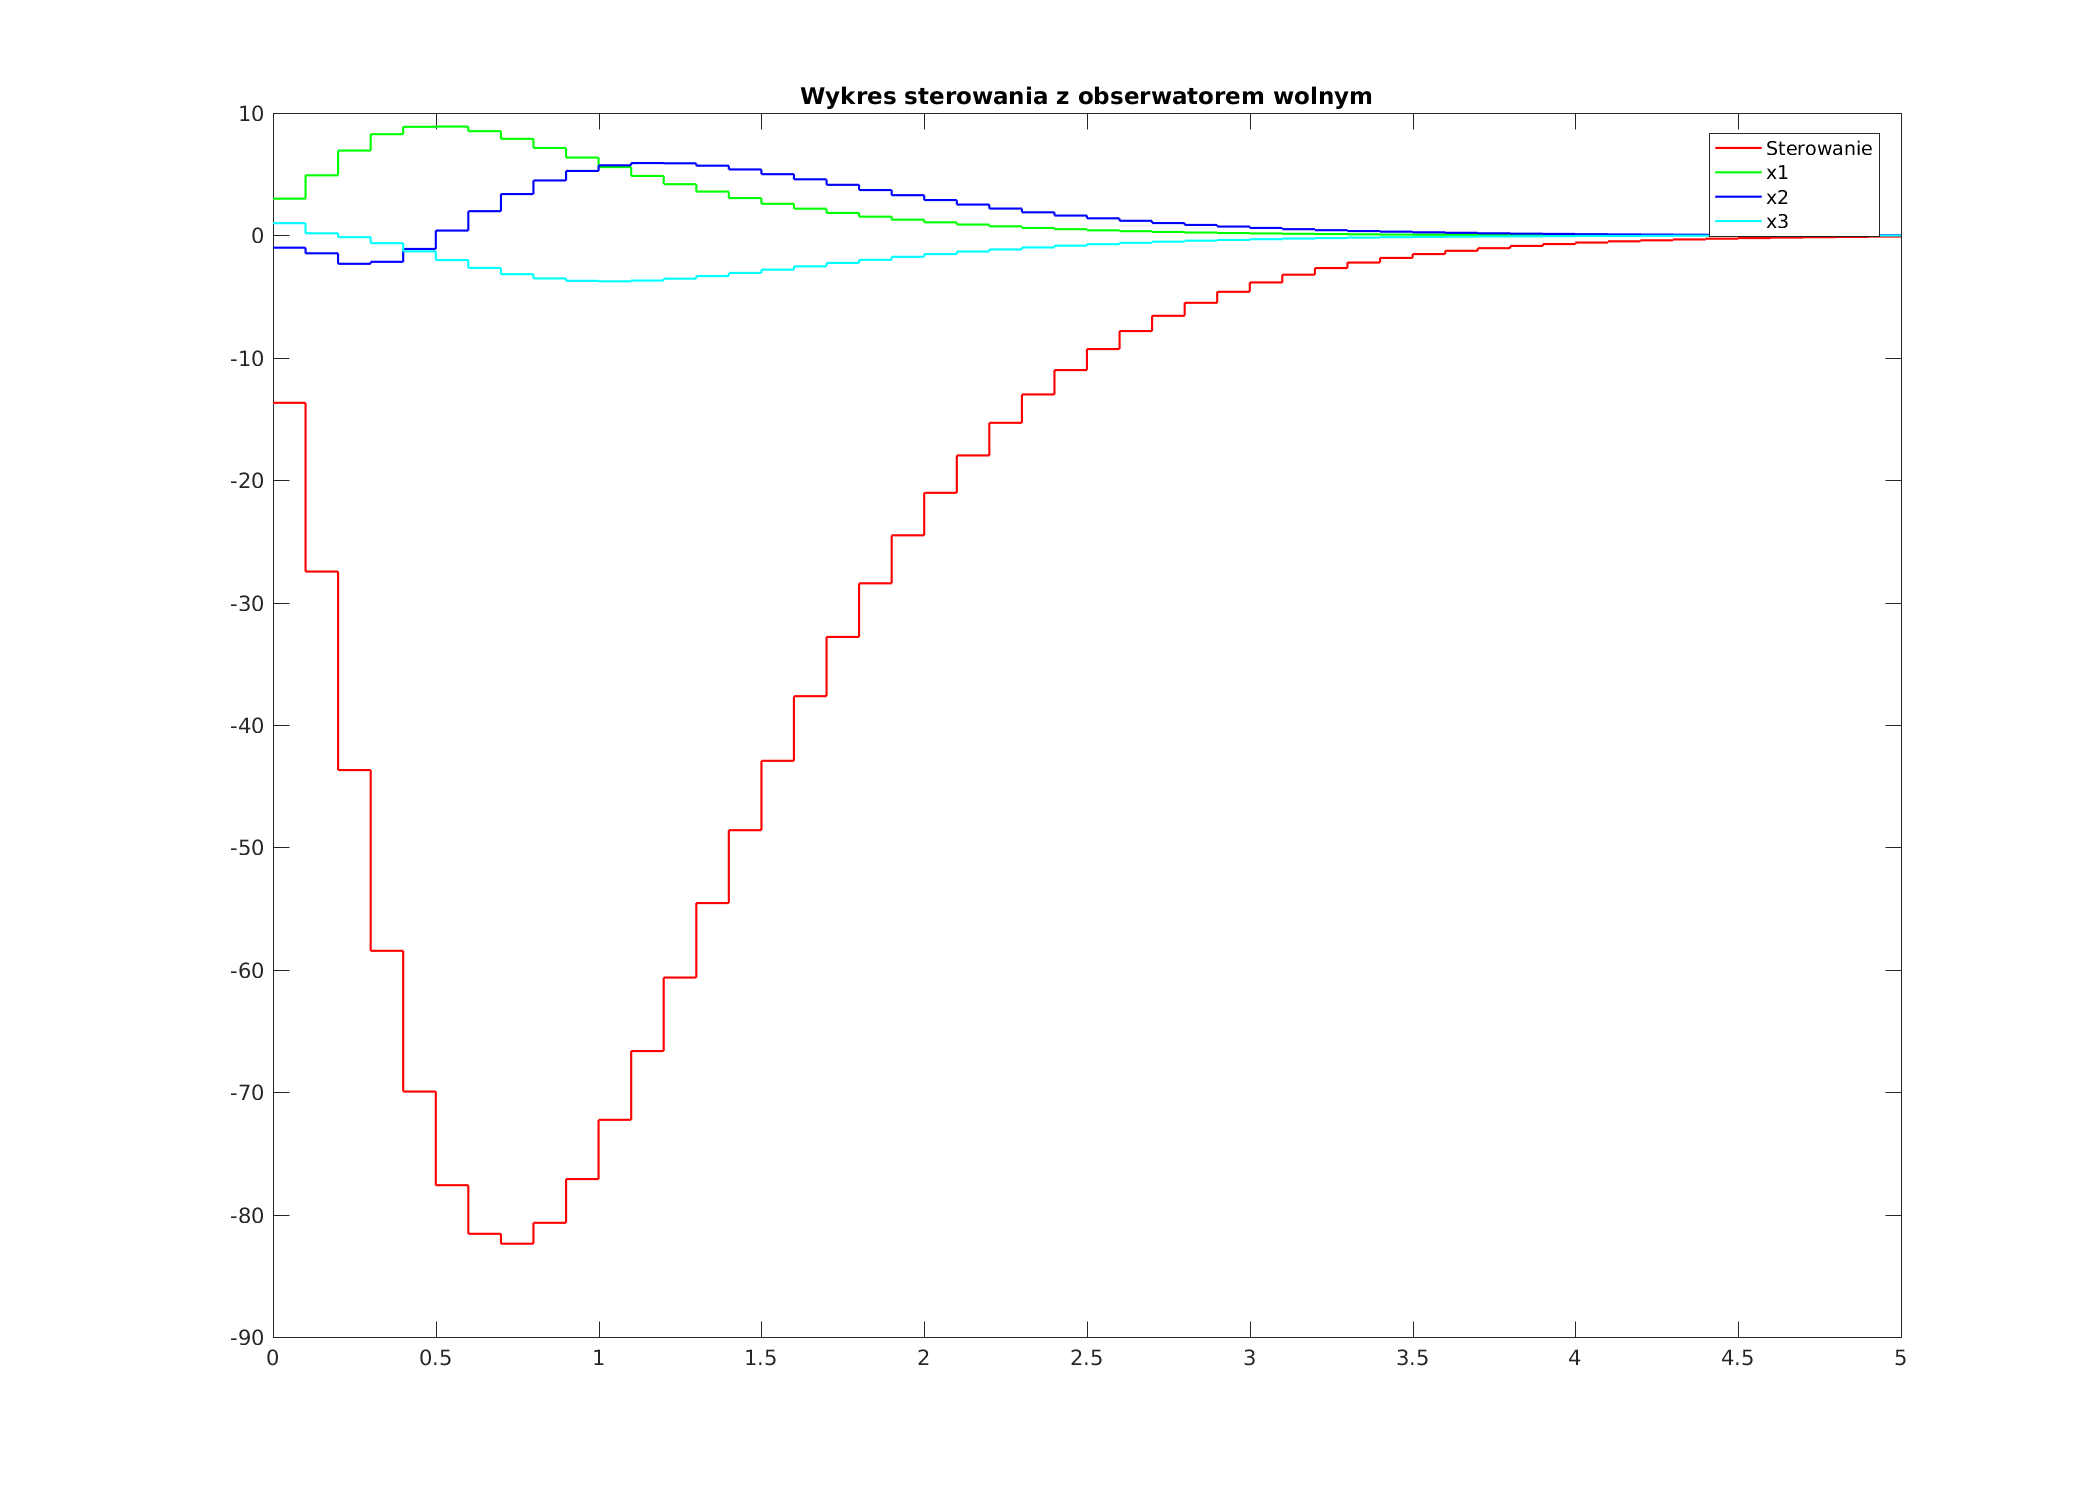
\includegraphics[scale=0.5]{4_a.png}
\caption{Symulacja modelu z obserwatorem wolnym}
\end{figure}

\subsection{Obserwator szybki}
W kolejnym podpunkcie należało tak ulokować bieguny obserwatora, aby regulacja następowała szybko. Dodatkowym wskaźnikiem jakośći podczas obsewacji była umiarkowana wartość sygnału sterującego. Najlepszy rezultat z symulowanych wystąpił dla wektora: \\

$p = [0.3\quad0.3]$\\

\begin{figure}[H]
\centering
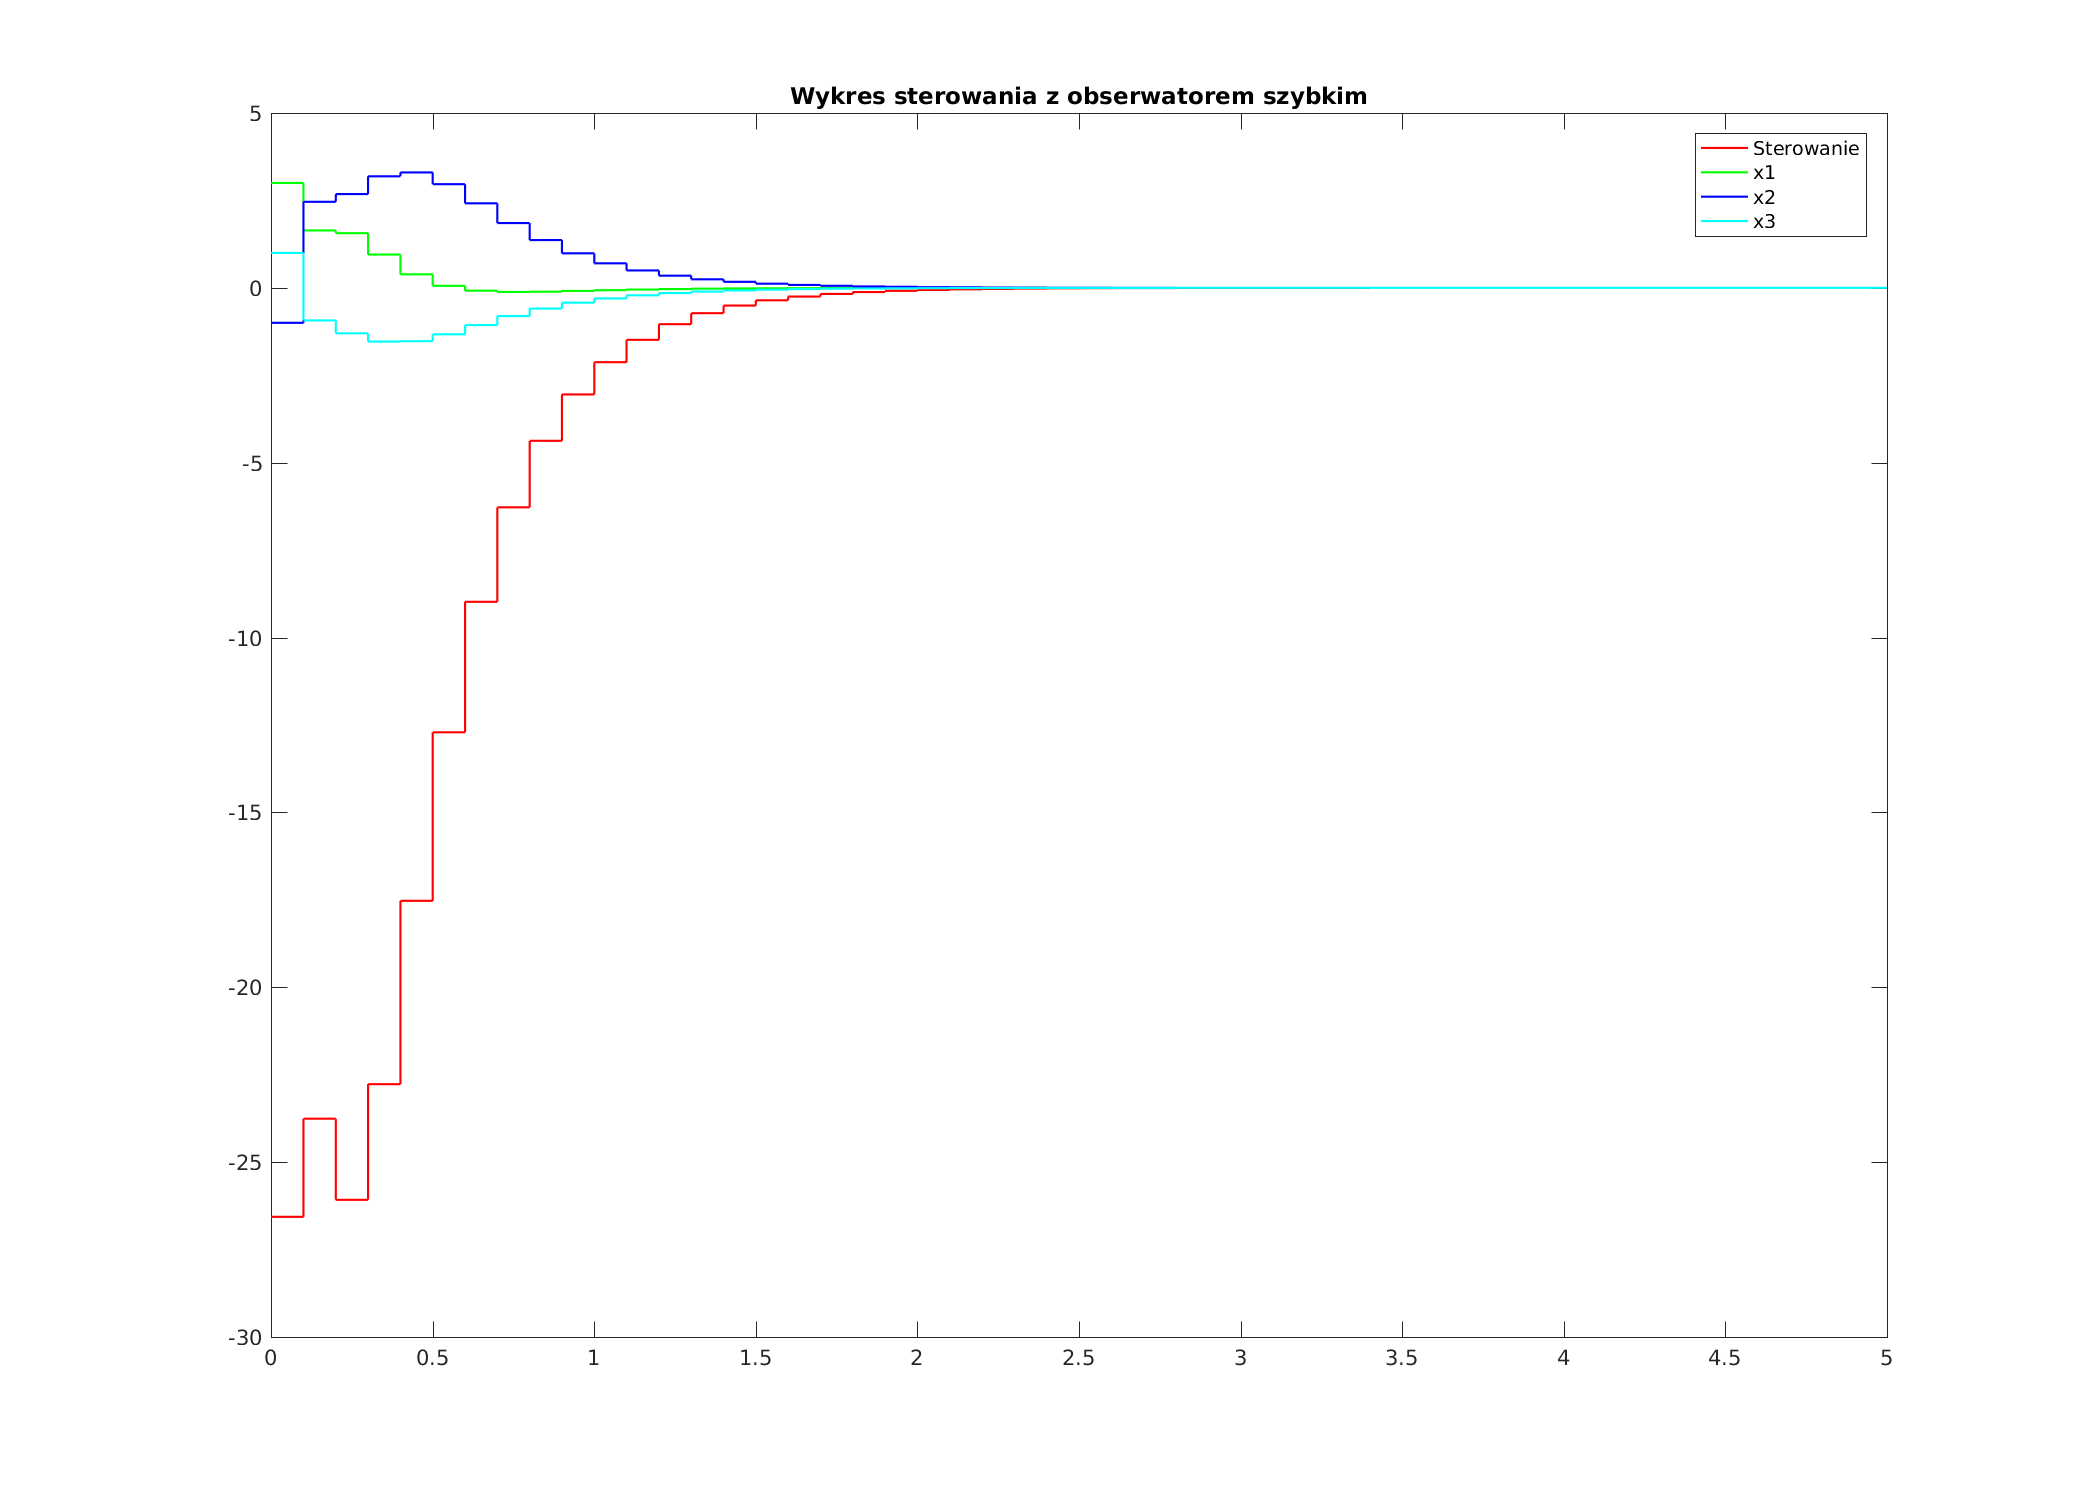
\includegraphics[scale=0.5]{4_b.png}
\caption{Symulacja modelu z obserwatorem szybkim}
\end{figure}














      




\end{document}